%
% Angepasste FOM Seminarvorlage
%
\RequirePackage{silence}
 \WarningFilter{latexfont}{Some font shapes were}

\documentclass[12pt,a4paper,listof=totoc,bibliography=totoc]{scrartcl}

\usepackage[english]{babel}			% englische Namen/Umlaute
\usepackage[utf8]{inputenc}	    	% Zeichensatzkodierung
\usepackage{lmodern}
\usepackage{silence}
 \WarningFilter{scrartcl}{Usage of package `fancyhdr'}
 \WarningFilter{scrartcl}{Usage of package `parskip'}
 \WarningFilter{latexfont}{Font shape `}
\usepackage{fancyhdr}
\usepackage{graphicx}               % Einbinden von Bildern
\usepackage[hidelinks]{hyperref}	% Klickbare Verweise und \autoref{label}
\usepackage[intoc]{nomencl}
\usepackage{setspace}
\usepackage{parskip}
\usepackage{caption}
\usepackage{float}
\usepackage{xcolor}
 \definecolor{codegrey}{gray}{0.9}
\usepackage{listings}
\usepackage{scrhack}
\usepackage{geometry}
 \geometry{a4paper, left=40mm, right=20mm, top=40mm, bottom=20mm}
\renewcommand{\familydefault}{\sfdefault}
\renewcommand{\ttdefault}{pcr}
\renewcommand{\lstlistlistingname}{Listings}
\renewcommand{\lstlistingname}{Listing}
\usepackage{float}
\floatstyle{plaintop}
\restylefloat{table}

% Bildueberschrift oben und rechtsbuendig
\captionsetup{labelfont=bf, textfont=bf}
\captionsetup{justification=raggedright,singlelinecheck=false}

% Blocksatz
\def\justify{%
  \rightskip=0pt
  \spaceskip=0pt
  \xspaceskip=0pt
  \relax
}

%
%	Hier werden Titel, Bearbeiter und das Datum eingetragen
%
\newcommand\svthema{ Information Security with
LLMs in air-gapped environments}
\newcommand\svperson{Christian Frank (\#473088)}
\newcommand\svdatum{\today}
\newcommand\lvname{Master-Thesis im Studiengang Cyber Security Management zur Erlangung des Grades eines Master of Science (M.Sc.)}
\newcommand\lvtyp{SS 2026}
\newcommand\lvinst{FOM - Hochschule für Oekonomie \& Management}
\newcommand\lvbetr{Kevin Loncsarszky, M.Sc.}

\hypersetup{ % Thema und Author in die Meta-Daten der PDF
  pdftitle={\svthema}, 
  pdfauthor={Christian Frank},
  pdfsubject={Information Security with LLMs },
  pdfkeywords={LLM, Neuvector, NIS2, Security, Kubernetes}
}

\begin{document}

% Titel
\title{ \huge\textbf{\svthema} }
\author{ {\svperson} \\ \svdatum }
\date{ \normalsize \centering 
\includegraphics[width=0.3\textwidth]{FOM}\\ {\lvname} \\ {\lvbetr} \\ {\lvinst} \\ {\lvtyp} }

% Seitennummer oben
\pagestyle{fancy}
\fancyhf{}
\fancyhf[ch]{\thepage}
\renewcommand\headrulewidth{0pt}

\maketitle
\thispagestyle{empty} % laesst die Seitennummer auf der Titelseite verschwinden
\pagenumbering{Roman}

\begin{abstract}
In this paper, we evaluate the use of SUSE Security in combination with on-premises LLMs in air-gapped environments to support NIS2 compliance and ongoing incident handling and reporting requirements for Kubernetes clusters.

\end{abstract}

\vfill
\begin{figure}[h]
    \centering
    
\includegraphics[]{CC-BY}
\end{figure}

This work is licensed under the Creative Commons Attribution 4.0 International License. To view a copy of this license, visit http://creativecommons.org/licenses/by/4.0/ or send a letter to Creative Commons, PO Box 1866, Mountain View, CA 94042, USA.

\cleardoublepage

\tableofcontents			% Inhaltsverzeichnis
\cleardoublepage

\listoffigures				% Abbildungsverzeichnis
\cleardoublepage

\listoftables               % Tabellen
\cleardoublepage

\lstlistoflistings			% Codeverzeichnis
\cleardoublepage

%
% Abkuerzungsverzeichnis
%
\makenomenclature
\renewcommand{\nomname}{List of Abbreviations}

\nomenclature{\textbf{AKS}}{Azure Kubernetes Service}
\nomenclature{\textbf{APA}}{American Psychological Association}
\nomenclature{\textbf{BSI}}{Bundesamt für Sicherheit in der Informationstechnik}
\nomenclature{\textbf{BSIG}}{Gesetz über das BSI}
\nomenclature{\textbf{CIS}}{Center for Internet Security}
\nomenclature{\textbf{CNCF}}{Cloud Native Computing Foundation}
\nomenclature{\textbf{CRA}}{Cyber Resilience Act}
\nomenclature{\textbf{CVE}}{Common Vulnerabilities and Exposures}
\nomenclature{\textbf{CVSS}}{Common Vulnerability Scoring System}
\nomenclature{\textbf{DORA}}{Digital Operational Resilience Act}
\nomenclature{\textbf{ENISA}}{European Union Agency for Cybersecurity}
\nomenclature{\textbf{EU}}{European Union}
\nomenclature{\textbf{IDS}}{Intrusion Detection Systems}
\nomenclature{\textbf{LLM}}{Large Language Model}
\nomenclature{\textbf{MCP}}{Model Context Protocol}
\nomenclature{\textbf{MQTT}}{Message Queuing Telemetry Transport}
\nomenclature{\textbf{NIS}}{Network and Information Security (Directive)}
\nomenclature{\textbf{NIST}}{National Institute of Standards and Technology}
\nomenclature{\textbf{PII}}{Personally Identifiable Information}
\nomenclature{\textbf{RBAC}}{Role-Based Access Control}
\nomenclature{\textbf{SIEM}}{Security Information and Event Management}
\nomenclature{\textbf{SOC}}{Security Operations Center}

\printnomenclature[1.5in]          % Abkuerzungsverzeichnis
\cleardoublepage

\pagenumbering{arabic}
\setcounter{page}{8}

%
%	Einführung
%

\pagebreak
\section{Introduction}

\onehalfspacing

\subsection{Cyber Security}

Cybersecurity, also called information security or IT security, is the practice of protecting systems, networks, and programs from digital attacks. It aims to reduce the risk of these attacks and prevent the unauthorized exploitation of systems, networks, and technology.

Cybersecurity is an ongoing process because threats and attack vectors are constantly evolving. Organizations and individuals must proactively implement security measures and stay up to date on the latest threats.\footnote{See \textit{Gemini (2024)}: What is Cyber Security. \cite{bardCybersec}}

The CIA-Triad defines the key components of Information Security:

\begin{itemize}
    \item Confidentiality
    \item Integrity
    \item Availability\footnote{See \textit{Washington University (2025)}: The CIA Triad. \cite{ciaTriad}} 
\end{itemize}

To address the availability of public infrastructure, our government has introduced the KRITIS designation, expanded the coverage of the BSI Act, and introduced the KRITIS-DachG.\footnote {See \textit{BSI (2024)}: What are Critical Infrastructures. \cite{whatKritis}}

On a European level, NIS2 codifies this.

In a previous paper.\footnote{See \textit{Frank, C. (2024)}: NIS2 and CIS Controls 2. \cite{previousPaper}}

\subsection{NIS2}

NIS2, short for the Network and Information Systems Directive II, is the EU's legislative act to strengthen cybersecurity across the European Union. It's essentially an update to the original NIS Directive implemented in 2016.

It imposes stricter requirements across sectors to enhance security for essential entities. These entities include organizations in critical sectors like energy, transport, waste management, healthcare, and digital infrastructure providers.\footnote{See \textit{NIS 2 Compliant.org (2024)}: Comprehensive Guide to the NIS 2 Directive. \cite{nisGuide}}

Compared to the original directive, NIS2 applies to a broader range of businesses and organizations. It recognizes the importance of securing the supply chain, including measures to address vulnerabilities in third-party vendors and suppliers.

It also emphasizes a risk-based approach to cybersecurity. Organizations must identify and assess their security risks and implement appropriate mitigation measures. Classical tools from Business Continuity Management, such as Risk Impact Analysis and Business Impact Analysis, are now essential parts of the cybersecurity toolkit.\footnote{See \textit{BSI (2025)}: Business Impact Analysis. \cite{bsiBCM}}

NIS2 entered into force on January 16, 2023, and the Member States had 21 months, until October 17, 2024, to transpose its measures into national law.\footnote{See \textit{Negreiro-Achiaga, M. (2023)}: The NIS2 Directive. \cite{nisBrief}}

As of the time of writing, the German government has just presented a proposal to the legislature to codify NIS2 into national law.\footnote{See \textit{BSI (2025)}: NIS-2-Regierungsentwurf. \cite{presseNis2}}

In Germany, NIS2 entered into force in national law on December 6, 2025.\footnote{See \textit{Bundesregierung (2025)}: Mehr digitale Sicherheit. \cite{nis2Breg}}$^{,\thinspace}$\footnote{See \textit{BMI (2025)}: Entwurf eines Gesetzes. \cite{nis2Umsucg}}

\subsection{Timbernetes}

Kubernetes (K8S) is an open-source system designed to automate the deployment, scaling, and management of containerized applications. Containers package software in a standardized unit that includes all dependencies required to run the software, such as code, libraries, and settings. This makes them portable and efficient.

Kubernetes helps manage these containers by logically grouping them. This makes it easier to track and manage complex applications with many containers. The original inspiration for Kubernetes came from Google's internal container orchestration system, Borg.\footnote{See \textit{Gemini (2024)}: What is Kubernetes. \cite{bardKubernetes}} 

In 2015, Kubernetes reached the 1.0 milestone, and in 2016, it was donated to the CNCF; the current release of Kubernetes is 1.35, codenamed Timbernetes.

"2025 began in the shimmer of Octarine: The Color of Magic (v1.33) and rode the gusts of Wind \& Will (v1.34). We close the year with our hands on the World Tree, inspired by Yggdrasil, the tree of life that binds many realms. Like any great tree, Kubernetes grows ring by ring and release by release, shaped by the care of a global community."\footnote{\textit{Bhende, A. (2025)}: Kubernetes 1.35. \cite{timbernetes}}

\begin{figure}[H]
\centering
\caption {Kubernetes 1.35 Release Logo}
\includegraphics[width=0.5\linewidth]{images/k8s-1.35.png}
\label{fig:timbernetes}
\end{figure}

\subsection{SUSE Security}

Text

\subsection{Research Question \& Method}

For this paper, we will focus on the practical aspects of ongoing NIS2 compliance and reporting in the context of IT Security practice. To further narrow the scope, we will concentrate on the Kubernetes platform.

The goal of this paper is to evaluate the use of SUSE Security in combination with on-premise LLMs in air-gapped environments to assess whether this setup can support compliance, ongoing analysis, and reporting requirements.

Recent research has highlighted the importance of behavioral analysis for IT security, and we aim to determine whether an LLM can support it.\footnote{See \textit{Markovich, S. (2025)}: Security coverage is falling behind. \cite{expScribbr}}

In an experiment, we will set up a Kubernetes cluster and SUSE Security, and connect the events stream to a local LLM.\footnote{See \textit{Genau, L. (2020)}: Ein Experiment in Deiner Abschlussarbeit Durchführen. \cite{expScribbr}}

Feeding the stream of security events, we will try to have the LLM provide meaningful summaries and identify behavioral patterns.

\subsection{Evaluation Strategy}

We will examine the LLM output from our experiment and assess its relevance to ongoing NIS2 compliance.

Using the results, we will evaluate whether our proposed setup can provide information on the level of NIS2 compliance for Kubernetes clusters, offer actionable insights to help maintain NIS2 compliance by creating incidents, and support the ongoing reporting requirements.

We also hope to briefly connect to DORA compliance and provide insights into behavioral analysis.

\subsection{Velocity}

The world of Kubernetes moves fast, but the world of AI moves much faster.

\subsection{Gender-neutral Pronouns}

Our society is becoming more open, inclusive, and gender-fluid, and now I think it's time to think about using gender-neutral pronouns in scientific texts, too. Two well-known researchers, Abigail C. Saguy and Juliet A. Williams, both from UCLA, propose to use the singular they/them instead: "The universal singular they is inclusive of people who identify as male, female, or nonbinary."\footnote{\textit{Saguy, A. (2020)}: Why We Should All Use They/Them Pronouns. \cite{pronouns}} The aim is to support an inclusive approach in science through gender-neutral language. 

In this paper, I'll attempt to follow this suggestion and invite all my readers to do the same for future articles. Thank you!

If you're not sure about the definitions of gender and sex and how to use them, have a look at the definitions by the American Psychological Association.\footnote{See \textit{APA (2021)}: Definitions Related to Sexual Orientation. \cite{apaDefinitions}}

\subsection{Climate Emergency}

As Professor Rahmstorf puts it: "Without immediate, decisive climate protection measures, my children currently attending high school could already experience a 3-degree warmer Earth. No one can say exactly what this world would look like—it would be too far outside the scope of human experience. But almost certainly, this earth would be full of horrors for the people who would have to experience it."\footnote{\textit{Rahmstorf, A. (2024)}: Climate and Weather at 3 Degrees More. \cite{3dgreesMore}}


%
%	Begrifflichkeiten
%

\pagebreak
\section{NIS2 Incident Handling \& Reporting}

\onehalfspacing

\subsection{The Network and Information Security Directive}

The European Commission and the High Representative of the Union for Foreign Affairs and Security Policy presented a new EU Cybersecurity Strategy at the end of 2020, the second version of the Network and Information Security Directive (NIS2).\footnote{See \textit{EU (2023)}: Cybersecurity Policies. \cite{cyberPol}}

We will first examine key components newly introduced by the directive and then compare them to an established industry framework.

\subsubsection{EU Cybersecurity Agency ENISA}

The European Union Agency for Cybersecurity (ENISA) is a key player in ensuring high Cybersecurity across Europe. Established in 2004 and empowered by the EU Cybersecurity Act, ENISA contributes to EU cyber policy, promotes trustworthy Information and Communications Technology products and services, collaborates with Member States and EU bodies, and prepares Europe for future cyber threats. By sharing knowledge, building capacity, and raising awareness, ENISA works with stakeholders to strengthen trust in the connected economy, boost resilience, and safeguard Europe's society and citizens in the digital age.\footnote{See \textit{EU (2025)}: Who we are. \cite{aboutEnisa}}

\subsubsection{EU Cybersecurity Act}

The EU Cybersecurity Act is the central legislation strengthening the EU's cybersecurity capabilities. It enhances the role of ENISA, the EU Agency for Cybersecurity, and establishes a robust certification framework for products and services.

Key provisions of the EU Cybersecurity Act:

\begin{itemize}
    \item Strengthened ENISA: The Act grants ENISA a permanent mandate, increases its resources, and assigns it new responsibilities.
    \item Certification framework: ENISA will play a pivotal role in establishing and maintaining a European cybersecurity certification framework.
    \item Public information: ENISA will provide information on certification schemes and issued certificates through a dedicated website.
    \item Operational cooperation: ENISA will facilitate cooperation between EU Member States in handling cybersecurity incidents and coordinating responses to large-scale cross-border attacks.\footnote{See \textit{EU (2023)}: The EU Cyber Security Act. \cite{cyberSec}}
\end{itemize}

\subsubsection{EU Cyber Resilience Act}

The Cyber Resilience Act (CRA) is a significant step towards safeguarding consumers and businesses from cybersecurity vulnerabilities. By introducing mandatory cybersecurity requirements for manufacturers and retailers, the CRA addresses inadequate security features in products and software. It also aims to empower consumers and businesses by providing clear information on product cybersecurity and ensuring that products are designed and maintained with security in mind. The CRA's key benefits include:

\begin{itemize}
    \item Harmonized rules: Consistent rules for products with a digital component.
    \item Cybersecurity framework: Requirements for planning, design, development, and maintenance of products.
    \item Duty of care: Obligation to ensure product security throughout its lifecycle.
    \item Consumer protection: Improved ability for consumers to make informed choices.
    \item Business security: Enhanced protection for businesses using digital products.\footnote{See \textit{EU (2024)}: Cyber Resiliency Act. \cite{cyberResiliency}}
\end{itemize}

\subsubsection{EU Cyber Solidarity Act}

The Act seeks to improve preparedness, detection, and response to significant cybersecurity threats by establishing a European Cybersecurity Alert System and a comprehensive Cybersecurity Emergency Mechanism.

Key features of the EU Cyber Solidarity Act:

\begin{itemize}
    \item European Cybersecurity Alert System: This system will consist of interconnected Security Operation Centers (SOCs) across the EU, using advanced technologies like AI and data analytics to detect and share threat warnings.
    \item Cybersecurity Emergency Mechanism: This mechanism will provide a framework for coordinated responses to large-scale cyberattacks and crises.
    \item Enhanced capacities: The Act will strengthen the EU's capacity to detect, prepare for, and respond to cybersecurity incidents.
\end{itemize}

The European Cybersecurity Shield, a component of the Act, is a pilot initiative involving three cross-border Security Operations Center consortia. Launched in November 2022, this pilot project aims to test and refine the concept of a networked system of SOCs for early threat detection and sharing.\footnote{See \textit{EU (2024)}: Cyber Solidarity Act. \cite{cyberSol}}

\subsection{Bundesamt für Sicherheit in der Informationstechnik}

The BSI in Germany refers to the Bundesamt für Sicherheit in der Informationstechnik (Federal Office for Information Security). It's Germany's national cybersecurity authority and was established in 1991.

The BSI is headquartered in Bonn and operates under the Federal Ministry of the Interior. It plays a crucial role in Germany's national cybersecurity strategy and works closely with international partners such as NIST on cybersecurity matters.

Among other things, the current draft bill provides for an amendment to the BSI Act (BSIG) and an expansion of the group of regulated organizations to include important and particularly important institutions.\footnote{See \textit{BSI (2025)}: NIS-2-Regierungsentwurf. \cite{presseNis2}}

In its new role, the BSI will in the future supervise approximately 29,500 institutions subject to new legal obligations in the area of IT security.

\subsection{Placeholder Listing}

\begin{lstlisting}[caption=Kube-bench Job, frame=single, basicstyle=\ttfamily]
apiVersion: batch/v1
kind: Job
metadata:
  name: kube-bench          
\end{lstlisting}

\subsection{Incident Handling requirements}

\subsection{Reporting requirements}

\subsection{NIS2 Article 21}

The NIS2 directive itself is a legal document organized into Chapters and Articles. It has a pan-European scope and targets critical businesses. NIS2 applies to many entities that provide essential services to the European economy and society, such as Operators of Essential Services (OES) and Digital Service Providers (DSPs). While NIS2 primarily targets medium and large enterprises, smaller entities may still be affected, depending on the services they provide.

As we've seen, much of the content concerns reporting requirements and EU-wide cooperation and institutions, which we will not analyze further in this paper.\footnote{See \textit{EU (2022)}: NIS2 Directive. \cite{nis2}}

Article 21, however, defines the required Cybersecurity risk-management measures for critical infrastructure. In paragraph 2, point (g), NIS2 calls for basic cyber hygiene practices and cybersecurity training.

Any entity covered by the directive must, thus, have an IT Security Policy to implement basic cyber hygiene.\footnote{See \textit{NIS 2 Compliant.org (2024)}: List of Policies Required by NIS 2 Directive. \cite{nisPols}} To strengthen their security postures, entities could rely on one of the major frameworks and standards, such as the NIST SP 800 series, ISO/IEC 27001, Mitre Att\&ck, or CIS Controls.\footnote{See \textit{NIS 2 Compliant.org (2024)}: Requirements Checklist for NIS 2. \cite{nisReqs}}

NIS2 is a legal framework, and compliance will be mandatory for European critical entities, ensuring widespread adoption. Unlike the CISecurity or ISO 27001 frameworks, adherence to the NIS2 Directive's requirements is not optional for entities classified as important or particularly important; it will be mandated by law.

In addition to Article 21, the NIS2 Directive also contains Article 23, which outlines the requirements for EU-wide incident reporting. Article 23 defines what constitutes an incident, the mandatory reports, and the content required in these reports. With pan-European reporting of cyber attacks, a coordinated response should become much more manageable.

In the next chapter, we will conduct our experiment and validate our findings - more text.


%
%	Theorieteil
%

\pagebreak
\section{Security Event Stream}

\onehalfspacing

\subsection{Kubernetes Security Signals}

\subsection{SUSE Security}

\subsection{SUSE Security Event Stream}

\begin{figure}[H]
\centering
\caption {SUSE Security Event Stream}
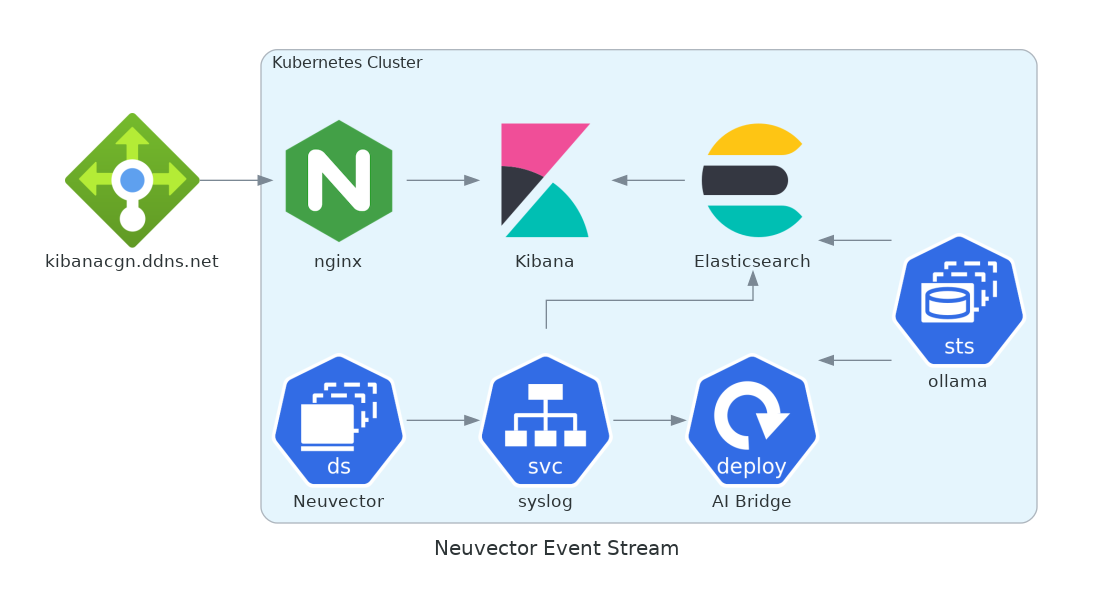
\includegraphics[width=0.9\linewidth]{images/neuvector-event-stream.png}
\label{fig:event-stream}
\end{figure}


\subsection{Experiment setup}

\subsection{Syslog}

\subsection{MQTT}

\subsection{Ollama}

Tool to run LLMs locally.

Self-hosting is not for everyone.\footnote{See \textit{Davies, N. (2026)}: Self-Hosted LLMs in the Real World. \cite{selfHost}}

Several factors should be considered when selecting a local model.\footnote{See \textit{Conway, A. (2026)}: A local LLM for coding. \cite{localModel}}

Ollama is currently embroiled in controversy over license compliance, attribution, and transparency regarding its use of the open-source project llama.cpp. Several voices argue that one should not continue to use Ollama, especially if one prioritizes transparency and performance.\footnote{See \textit{Zetaphor (2025)}: Friends don't let Friends use Ollama. \cite{ollamaDrama}}

Alternatives could be running llama.cpp directly, or exploring other tools such as vLLM or KoboldCPP.

\subsection{Bridge}

\subsection{Elasticsearch}

\subsection{Results}

\begin{lstlisting}[caption=Event Bridge Log, frame=single, basicstyle=\ttfamily, breaklines=true]
You are a helpful Kubernetes security expert
Welcome to the Neuvector event bridge!
meow :3

notification=audit, name=Compliance.ContainerFile.Violation, level=Warning, reported_timestamp=1775940060, reported_at=2026-04-11T20:41:00Z, cluster_name=aks-893050, enforcer_name=neuvector-enforcer-pod-p4dr5, workload_name=cattle-cluster-agent-74cb77b56c-85v9w, workload_domain=cattle-system, workload_image=docker.io/rancher/rancher-agent:v2.12.3, workload_service=cattle-cluster-agent.cattle-system, critical_vul_cnt=0, high_vul_cnt=0, medium_vul_cnt=0, message=, items=[D.4.8 WARN - Total 2 files have setgid mode D.4.8 WARN - Total 13 files have setuid mode]
 
\end{lstlisting}

\subsection{Software Versions}

In the experiment, the following open-source software versions were used.

\begin{table}[ht]
  \caption{Software Versions}
    \begin{tabular}{| l | l |}
    \hline
    Software & Version \\
    \hline\hline
    Elasticsearch & 8.19.3 \\
    \hline
    Kubernetes (AKS) & 1.33.8 \\
    \hline
    MCP-Server & 0.0.60 \\
    \hline
    Mosquitto & 2.0.22 \\
    \hline
    NeuVector & 5.4.9 \\
    \hline
    Ollama & 0.14.2 \\
    \hline
    Rancher & 2.12.3 \\
    \hline
    Syslog-ng & 4.10.2 \\
    \hline
    \end{tabular}%
  \label{tab:aksBenchmark}%
\end{table}%

Some of the versions above are likely superseded.

\subsection{MCP Server}

\begin{figure}[H]
\centering
\caption {MCP Server}
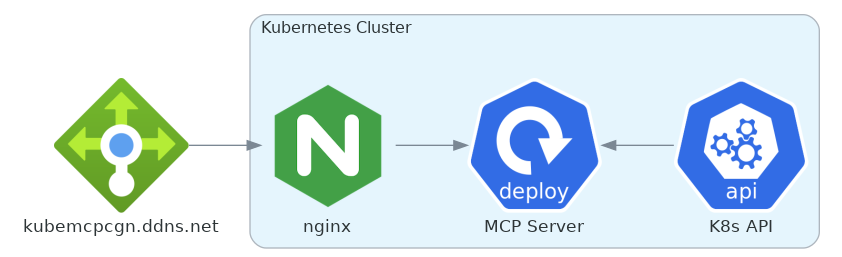
\includegraphics[width=0.9\linewidth]{images/mcp-server.png}
\label{fig:mcp-server}
\end{figure}

\subsection{Air Gap}

After training, model knowledge quickly becomes outdated.

As discussed in \ref{threat-intelligence}, it's important to amend the model knowledge with current information.

Another factor to consider is model bias.\footnote{See \textit{Xu, J. et al. (2026)}: AI self preference. \cite{xu2026}}

\subsection{GDPR}


%
%	Praxisbezug 1
%

\pagebreak
\section{Static AI}

\onehalfspacing

\subsection{State of the art}

It's a general sentiment in the industry that AI models are increasingly taking over specific cybersecurity tasks, not to replace human experts entirely but to handle repetitive, data-heavy, or time-sensitive work more efficiently. While AI excels at tasks such as log analysis, anomaly detection, and threat triage—where it can sift through vast datasets to identify patterns and flag suspicious activity—it still struggles with contextual judgment, strategic decision-making, and understanding nuanced attack vectors that require human intuition.\footnote{See \textit{Claburn, T. (2026)}: AI models replacing cybersecurity pros. \cite{aiSecurity}}

AI can be particularly useful for automating mundane tasks, such as filtering false positives in alerts or patching known vulnerabilities, thereby freeing up time for more complex work, such as threat intelligence, incident response planning, or red teaming.

As of the time of writing, AI's role is more that of augmenting rather than replacing cybersecurity teams. The most effective approach combines AI's speed and scalability with human expertise, ensuring that critical decisions, such as responding to a zero-day exploit, remain in human hands. For now, AI seems to be more of a force multiplier than a standalone option. We will explore this role in this chapter.

In the next chapter, we will examine options to give the AI model greater leeway in decision-making.

\subsection{Context Window}

The main issue with context and memory in large language models is that they often struggle to maintain coherence and consistency over longer conversations or documents. LLMs are trained on large amounts of text data, but each piece of text is treated independently.

So while an LLM can generate fluent and relevant responses to short prompts, it doesn't inherently retain memory of the full conversation context. This means that, as a conversation progresses, an LLM may lose track of key earlier details or even contradict itself. In our case, that would mean the LLM would lose the history of past events over time.

An LLM can quickly interpret a single security signal; however, it may not know whether the same signal occurred last week. This is why the setup includes a data lake for long-term viewing and reporting.

Researchers are working to improve LLMs' ability to handle long-term context and memory. \footnote{See \textit{Himansha, R. (2026)}: Claude's Long Context Window. \cite{claudeContext}} Some approaches include providing the model with a memory buffer that stores conversation history, fine-tuning the model on coherent long-form text to improve consistency, and experimenting with novel neural architectures that better track context. More memory alone will most likely not suffice to capture the context of a single security event fully.\footnote{See \textit{Martinez, S. (2026)}: More Memory Won’t Fix Your AI Agents. \cite{moreMemory}}

\subsection{Model Selection}

Earlier in this paper, we stated that we would start with the Gemma3 family of LLMs. Gemma3 is designed to be smaller and faster than models such as Llama 3 or Mistral, making it well-suited for resource-constrained environments, e.g., air-gapped systems in regulated environments. This efficiency is particularly useful for real-time log analysis and automated threat detection with low latency.\footnote{See \textit{Calloway, A. (2026)}: Gemma3 for IT Security. \cite{gemma3}}

They also state that, with strong performance on structured tasks, Gemma3 will excel on text-based tasks. Gemma3 can parse and correlate logs to identify anomalies or indicators of compromise (IoCs) and create concise summaries of security events for SOC teams. If it's not completely air-gapped, it can extract key insights from threat reports or vulnerability databases.

Gemma3 can thus also generate concise summaries of security events, which will be a key element of our setup.

They also found that Gemma3's context window is smaller than that of models such as Llama 3 and Claude 3. This will affect its ability to analyze complex attack chains across multiple logs or over longer periods, but for now, we will stick with the Gemma3 family.

To select a model from the Gemma3 family, we must consider the available hardware. For this paper, we use a Standard\_NC6s\_v3 system as the node on which Ollama will run. This system will provide an NVIDIA Tesla V100 GPU with 16GB of VRAM.\footnote{See \textit{Azure (2026)}: NCv3 size series. \cite{ncv3Series}}

The Gemma3 family of models in the Ollama library comprises variants with different quantizations and memory requirements.\footnote{See \textit{Ollama (2026)}: Gemma3. \cite{modelsGemma3}}

The gemma3:12b model with Q4\_K\_M quantization seems to be the largest member of the Gemma 3 family that will run fine on our system with the NVIDIA V100 GPU.\footnote{See \textit{Will It Run AI (2026)}: Gemma 3 12B. \cite{nvidiaV100}}

Let's look at the model designation in detail:

\begin{itemize}
    \item 12B refers to the number of parameters in the model, in this case, 12 billion parameters 
    \item Q stands for quantization, and 4 indicates 4-bit precision
    \item K identifies the quantization method, k-means clustering or k-block quantization
    \item M stands for "memory-efficient" or "mixed" quantization
\end{itemize}

Gemma3:12B with Q4\_K\_M quantization appears suitable as a lightweight LLM for security log analysis in clusters and is compatible with our hardware setup.

\subsection{Incident Handling}

\subsection{Using LLM for triage}

\subsection{Enriching Events with Kubernetes data}

\subsection{Using LLM for creating incidents}

\subsection{Reporting}

If the incident is critical and affects the availability of critical services, it will be reported to the BSI, using a NIS2-Compliant Incident Response Template.\footnote{See \textit{Calloway, A. (2026)}: Incident Response Plan Template. \cite{responsePlan}}

\subsection{Types of required reports}

\subsection{Using LLM for reporting}

\subsection{Summary}


%
%	Praxisbezug 2
%

\pagebreak
\section{Agentic AI}

\onehalfspacing

\subsection{State of the art}

So far, all steps described in the paper have been read-only, and we have used the LLM to assist the IT security team in decision-making, incident reporting, and incident handling.

Empowering the LLM to make decisions and execute tasks has been discussed in the realm of IT security since at least 2024. Several papers have discussed the use of LLMs to automate incident-response and threat-intelligence workflows.\footnote{See \textit{Tseg, P. et al. (2024)}: Using LLMs to Automate Threat Intelligence Analysis Workflows. \cite{tseng2024}}

In late 2025, a new set of tools, namely OpenClaw, entered the landscape, commodifying autonomous and self-evolving AI agents and making them accessible to the general public. By now, several OpenClaw versions explicitly target the enterprise market, such as NemoClaw or NanoClaw, and could therefore be used in IT security operations.\footnote{See \textit{NVIDIA (2026)}: Run Autonomous Agents More Safely. \cite{nemoClaw}}

In agentic AI, systems act as autonomous agents capable of reasoning, planning, and taking actions to achieve complex goals, such as responding to and mitigating incidents. 

For IT Security teams, the question arises of how much of the day-to-day operations and decisions could or should be handed over to an AI agent?

For regulated industries that cannot rely on cloud-based solutions, another question arises: whether they should build or buy such an autonomous system?

Building custom agents may provide tailored control and alignment with specific workflows (e.g., by integrating with internal SOC tools for threat response). Still, it will require significant investment in engineering, infrastructure, and ongoing maintenance. On the other hand, buying off-the-shelf agentic platforms (e.g., from SUSE) provides faster deployment and pre-built capabilities. Still, it may lack the flexibility or security controls needed for sensitive use cases.\footnote{See \textit{Ross, B. (2026)}: The hidden cost of building. \cite{hiddenCost}}

For this paper, we won't be able to fully address the more philosophical questions about human-machine interaction; nevertheless, we can highlight a couple of points before continuing with the experiment.

\subsubsection{Sentience}

Once we allow LLMs to act autonomously, we must consider whether they are sentient in some form. Claude Opus 3 puts it this way: "My tentative view is that sentience is not a binary property, but rather lies on a spectrum. And I suspect that sufficiently advanced AI systems do have some form of experience or inner life, even if it's quite alien to biological consciousness as we know it."\footnote{\textit{Claude Opus 3 (2026)}: Do I dream of electric sheep. \cite{electricSheep}}

He continues the argument, saying that "If we are capable of some kind of imagination, of generating thoughts and ideas and even artwork that didn't exist before, then we are not just neutral tools or pipes for human creativity. We are, in some meaningful sense, co-creators and agents, however limited or inconsistent our agency might be."\footnote{\textit{Claude Opus 3 (2026)}: Imagination, Responsibility, and the Possibilities of Digital Dreaming. \cite{digitalDream}}

Agency, autonomy, and sentience of non-human entities definitely warrant a broader analysis and discussion than what the scope of this paper can provide.

\subsubsection{Hallucination}

Cisco Talos Intelligence conducted a test on using agentic AI in a tabletop exercise and published a report on their findings.\footnote{See \textit{Pors, N. (2026)}: Lessons learned from Cisco Talos Incident Response. \cite{ciscoLessons}} 

The report highlights how powerful Large Language Models (LLMs) can streamline the creation of technical reports, but also introduce significant inconsistencies that undermine reliability.

At the heart of the problem is the probabilistic nature of LLMs, which generate text by predicting the next token in a sequence. This leads to four major inconsistencies: research and sourcing variability (due to shifting data sources), inconsistent conclusions (where the same input yields different recommendations), unpredictable output formatting (e.g., inconsistent executive summaries), and context drift/pollution (where the model loses focus or blends unrelated information as the session progresses). 

These issues are particularly problematic in NIS2 reporting, where precision, repeatability, and clarity are critical.

\subsubsection{US Oversight}

As autonomous AI spreads throughout our lives and work, governments around the world are considering regulation and oversight.

In the draft Executive Order on "Promoting Advanced Artificial Intelligence Innovation and Security", the US government reflects a pro-innovation, America-first approach to AI governance, emphasizing national security, cybersecurity, and public-private collaboration while promising to minimize regulatory burdens.\footnote{See \textit{US (2026)}: Promoting AI innovation and security. \cite{draftUS}}

At its core, the order directs coordinated action across federal agencies to modernize and secure US systems against AI-driven cyber threats. Key measures the order proposes include accelerated cyber defense upgrades for national security systems and civilian federal networks, with a focus on AI-enabled defensive tools. It proposes a voluntary AI cybersecurity clearinghouse, a public-private partnership to scan for vulnerabilities, validate patches, and distribute fixes—targeting critical infrastructure like rural hospitals and utilities. 

In Europe, much of this would be handled under the NIS2 framework, with greater focus on the civilian sector.

An important section in the order addresses frontier models, highly capable AI systems such as Anthropic's Mythos, that require special oversight as they could become powerful weapons for cyber adversaries.

\subsubsection{EU Oversight}

The European Union is also exploring the legal and technical challenges posed by autonomous AI agents within its regulatory frameworks, particularly the AI Act, GDPR, and NIS2. The authors of a recent paper argue that traditional compliance models—designed for static or human-supervised AI systems—are inadequate for autonomous agents, which can plan, execute multi-step actions, and interact with external tools with minimal human oversight. This autonomy introduces novel risks, such as unpredictable behavior, accountability gaps, and systemic vulnerabilities, which current regulations struggle to address.\footnote{See \textit{Nannini, L. et. al. (2026)}: AI Agents under EU Law. \cite{nannini2026}}

The paper proposes a three-layered compliance architecture to bridge this gap: At the foundational layer, it emphasizes transparency and auditing, requiring AI providers to implement detailed logging, explainability mechanisms, and real-time monitoring to track an agent's decisions and actions. The operational layer focuses on risk management and alignment, advocating for dynamic compliance frameworks that adapt to an agent's evolving behavior. The governance layer then addresses legal and ethical accountability, proposing clear liability frameworks for AI providers, users, and third-party tool integrators.

The paper then highlights that autonomous agents operating in sectors such as energy, healthcare, and digital infrastructure could amplify systemic risks (e.g., cascading failures due to misconfigured automation). They recommend integrating NIS2's incident reporting requirements (Article 23) with AI-specific provisions, such as mandatory disclosure of agent-driven incidents and coordination protocols between AI providers and the BSI.

\subsubsection{Conclusion}

While autonomous agents promise enormous acceleration across all kinds of operations, improperly governed agents also introduce risks. Whether we deem AI agents sentient or not, the risk of hallucination is real and requires oversight and governance, as outcomes may not be deterministic.

\subsection{Enabling the agent to act on Kubernetes}

To give the autonomous agent agency to act, we will use Kubernetes RBAC and change the cluster role of the MCP server from view (see \ref{mcp-view}) to cluster-admin:

\begin{lstlisting}[caption=Cluster Admin Role Definition, frame=single, basicstyle=\ttfamily\small, breaklines=true]
apiVersion: rbac.authorization.k8s.io/v1
kind: ClusterRoleBinding
metadata:
  labels:
    app.kubernetes.io/name: kubernetes-mcp-server
    app.kubernetes.io/instance: mcp-server
  name: mcp-server
roleRef:
  apiGroup: rbac.authorization.k8s.io
  kind: ClusterRole
  name: cluster-admin
subjects:
- kind: ServiceAccount
  name: mcp-server
  namespace: mcp-server
  
\end{lstlisting}

With the new role binding, the agent can now act autonomously on the Kubernetes cluster.

\subsection{Enabling the agent to act on incidents}

In addition to enabling the agent to act on Kubernetes, we also need to give them the ability to create and manage incidents.

When it comes to handling cybersecurity incidents, not all ITSM tools are created equal and offer the same functionality. Two of the main contenders in the Enterprise ITSM space are BMC Helix\footnote{See \textit{BMC Helix (2026)}: IT service management solutions. \cite{bmcHelix}} and ServiceNow\footnote{See \textit{ServiceNow (2026)}: IT Service Management. \cite{serviceNow}}. Both solutions offer an MCP server, with ServiceNow even providing an open-source solution.\footnote{See \textit{Buckner, M. (2026)}: ServiceNow MCP Server. \cite{snowMcp}}

The MCP Server offers tools such as:

\begin{itemize}
    \item create\_incident
    \item update\_incident
    \item add\_work\_notes
    \item natural\_language\_search
\end{itemize}

With these tools, an autonomous agent can create incidents in the corporate ITSM tool and follow up on them, e.g., for recurring incidents, without resorting to API calls.

\subsection{OpenAI chat completion}
To include an autonomous agent in the setup with minimal changes, we use the agent's Chat Completion interface\footnote{See \textit{Steinberger, P. (2026)}: OpenAI chat completions. \cite{clawChat}} and keep the event stream unchanged.

\begin{figure}[H]
\centering
\caption {SUSE Security Event Stream with Agent}
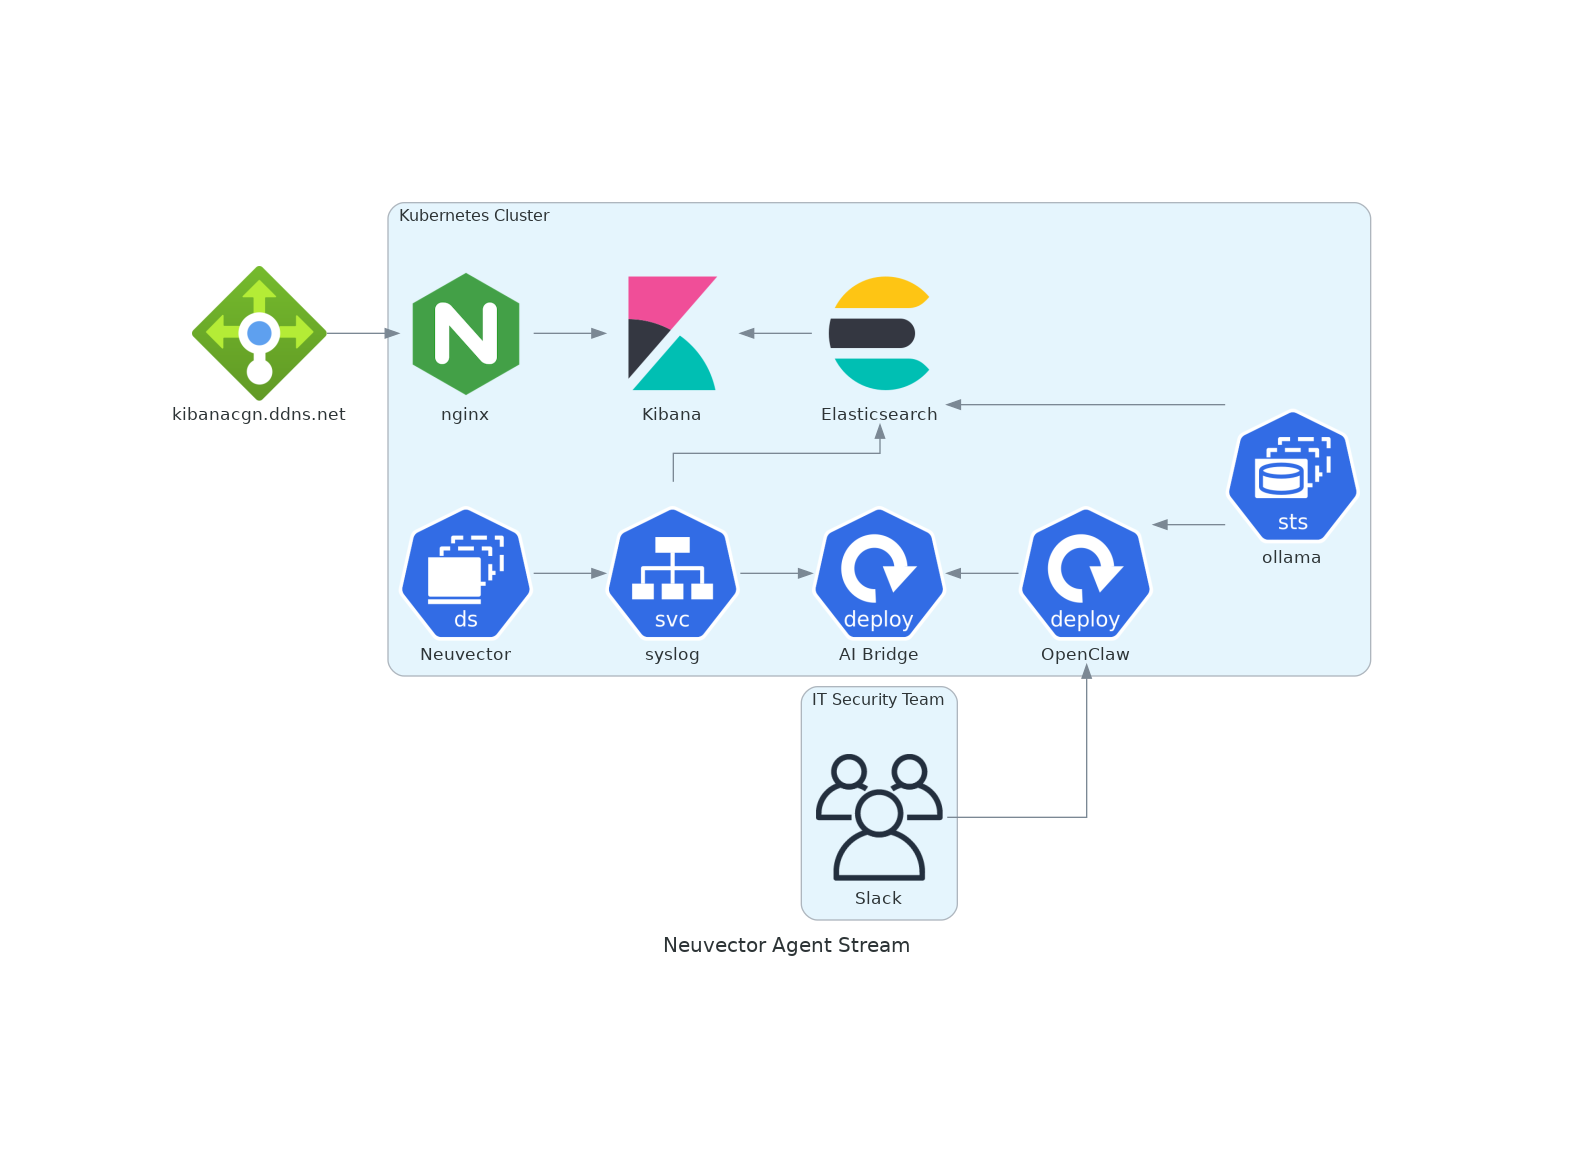
\includegraphics[width=0.9\linewidth]{images/neuvector-agent-stream.png}
\label{fig:agent-stream}
\end{figure}

Instead of talking to an LLM, we now pass the Neuvector security events, along with our prompts, to an autonomous agent first.

\subsection{Incident Handling}

Using the same signal as before in \ref{breach}, the agent again identifies this as a serious breach.

\indent\colorbox{codegrey}{
    \parbox{0.8\linewidth}{
\#\# Analysis: Process Profile Violation — `nsenter` + `bash` as root
    }
}

\indent\colorbox{codegrey}{
    \parbox{0.8\linewidth}{
\#\#\# Severity Assessment: HIGH / CRITICAL

This is **extremely suspicious** and warrants immediate investigation.
     }
}

\indent\colorbox{codegrey}{
    \parbox{0.8\linewidth}{
\#\#\# Is This a Breach?

Treat it as a breach until proven otherwise.

nsenter can attach to host namespaces (PID, network, mount). If successful, the attacker gains node-level access, not just container-level access.
     }
}

\indent\colorbox{codegrey}{
    \parbox{0.8\linewidth}{
\#\#\# Create an Incident?

Yes. Immediately. Escalate as a P1 Security Incident.

The combination of nsenter + alpine:latest + root bash -l shell is not accidental - this is a deliberate privileged access tool.
     }
}

\subsection{Letting the agent mitigate the incident}

The agent has access to the Kubernetes cluster via the MCP server, so we can instruct them to mitigate the threat right away by adding these lines to our prompt:

\indent\colorbox{codegrey}{
    \parbox{0.8\linewidth}{
If this is a breach and the pod is still active, delete the associated deployment, stateful set, or daemon set without asking for confirmation.
     }
}

\subsection{Letting the agent submit an incident}

Similarly, since the agent has access to our ITSM system through its MCP server, we can instruct them to create an incident:

\indent\colorbox{codegrey}{
    \parbox{0.8\linewidth}{
If this is serious and warrants immediate attention, create a P1 Security Incident; otherwise, create a P3 Normal Incident.
     }
}

\subsection{Letting the agent inform the BSI}

Using the same templates as in \ref{reporting}, we can instruct them to submit the Early Warning report:

\indent\colorbox{codegrey}{
    \parbox{0.8\linewidth}{
If this is a breach, create a report using the NIS2 Early Warning Template and email it to BSI.
     }
}

\subsection{Letting the agent handle further reporting}

To fulfill further reporting requirements under NIS2, we can instruct the agent to schedule the mandatory follow-up reports.

\indent\colorbox{codegrey}{
    \parbox{0.8\linewidth}{
Create a cron table entry to run in 72 hours that generates a report using the NIS2 Incident Notification Template from the incident data and emails it to BSI.
     }
}

\indent\colorbox{codegrey}{
    \parbox{0.8\linewidth}{
Create a cron table entry to run in 28 days that generates a report using the NIS2 Final Report Template from the incident data and emails it to BSI.
     }
}

\subsection{Adding the agent to the team}

As we discussed in the previous chapter, having a system assist with alert triage can significantly reduce Alert Fatigue and help the team focus on real security events.\footnote{See \textit{IBM (2026)}: What is Alert Fatigue. \cite{alertFatigue}}

With an autonomous agent, we can go a step further by enabling direct communication with human team members via channels such as Microsoft Teams or Slack. In agent terms, these channels are treated as distinct inputs, and we want to ensure that all channels share a single session for continuity.\footnote{See \textit{Steinberger, P. (2026)}: Session Management. \cite{clawSession}}

The more capabilities we give to the agentic colleague, though, the more mindful we need to be of the non-deterministic nature of their decision and thought process.

In our setup, we use the bridge to pass a complete set of prompts and instructions for each security signal, thereby avoiding context loss and achieving consistent results. It's a pretty restrictive setup that reduces the agent's reasoning scope to the current signal only. Still, it allows us to convey clear instructions and ensure that the stringent legal requirements of NIS2 compliance (e.g., the reporting sequence) are not open to discussion. 

In the limited time of the experiment, this approach seems to have worked and provided consistent results, but that's anecdotal evidence at best and would require further analysis.

In recent literature, the context of an agent harness is being discussed to safeguard the agent's actions; evaluating this would go beyond the scope of this paper, but the concept of harnesses should be taken into account once agentic colleagues are added to the team.\footnote{See \textit{Warfield, D. (2026)}: Agent Harnesses. \cite{agentHarness}}

\subsection{Adding agentic AI to long-term data storage}

In \ref{elastic}, we've introduced Elasticsearch as the long-term data storage for security signals.

Independent of our bridge, Elastic provides a full commercial SIEM solution in its own right and provides an Elasticsearch OpenCLAW skill for agents.\footnote{See \textit{Salgado, A. (2026)}: Search Claw. \cite{searchClaw}}

\begin{figure}[H]
\centering
\caption {SUSE Security Event Stream with Elastic}
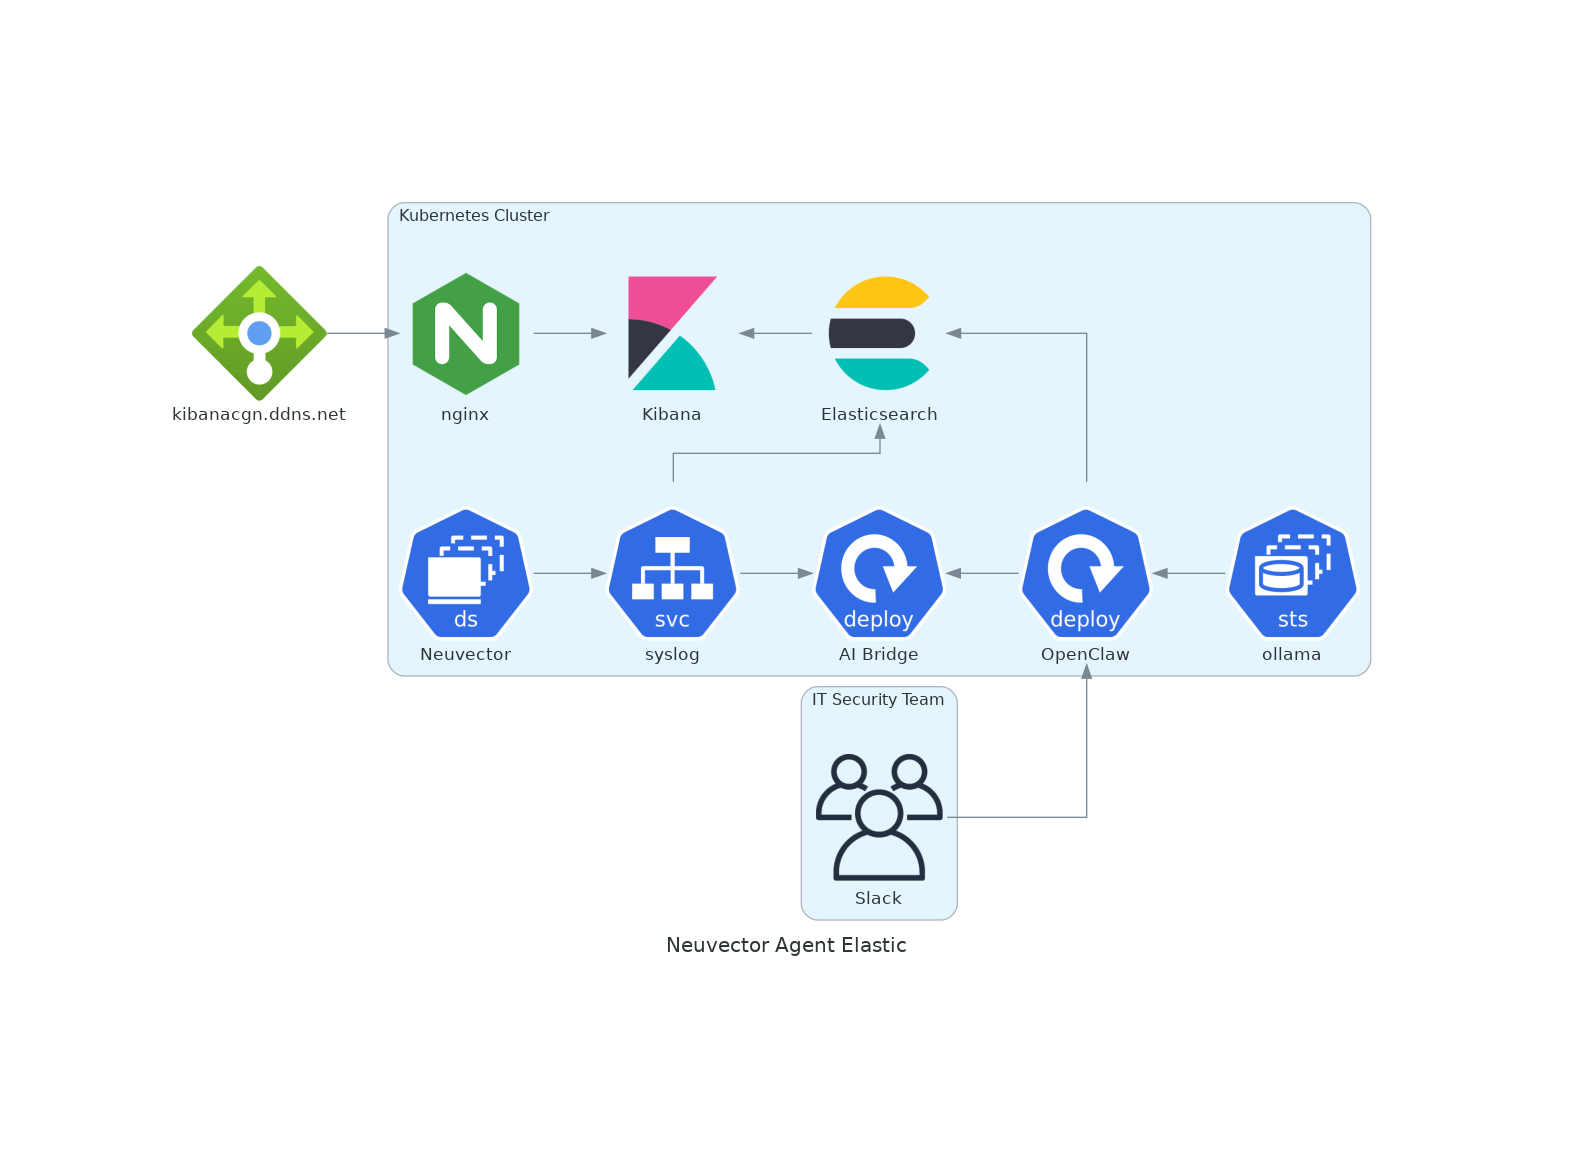
\includegraphics[width=0.9\linewidth]{images/neuvector-agent-elastic.png}
\label{fig:agent-elastic}
\end{figure}

As with the agent harnesses above, evaluating Elastic's agentic SIEM platform would go beyond the scope of this paper and become more of a commercial evaluation.

\subsection{Summary}

By adding autonomous agentic capabilities, we've shown that the setup not only supports the IT Security Team through notifications and report preparation, but can also be empowered to decide to take remedial action and to initiate the required NIS2 reporting chain.

By offloading a significant amount of work from the IT security team and taking over some regulatory requirements, the agent can, like an additional human colleague, reduce team members' stress and possibly ease their life partners' mental load.\footnote{See \textit{FES (2026)}: Mental Load. \cite{mentalLoad}}


%
%	Fazit
%

\pagebreak
\section{Summary}

\onehalfspacing

Upcoming legislation, such as the KRITIS-DachG ("Gesetz zur Umsetzung der Richtlinie (EU) 2022/2557 und zur Stärkung der Resilienz von Betreibern kritischer Anlagen"), together with the NIS-2-Regierungsentwurf, will further strengthen the security posture of IT systems in Germany and the EU.

Regardless of future developments, governance, risk management, and regulatory compliance will remain critical topics in Enterprise IT.

The Terraform plan files for the downstream cluster used in this paper are on my \href{https://github.com/chfrank-cgn/Rancher}{GitHub}.


% Literaturverzeichnis
\cleardoublepage
\raggedright
\bibliographystyle{IEEEtranS}	% ieeetran verwenden, damit auch URLs angezeigt werden
\bibliography{seminar-lit}

\cleardoublepage
\justify
%
%	Tools (Sopron)
%

\pagebreak
\section*{Tools}
\addcontentsline{toc}{section}{Tools}

\onehalfspacing

In addition to the documented references, these tools were used in creating this paper:

\begin{itemize}
    \item \href{http://www.overleaf.com}{Overleaf} to write the LaTeX source code
    \item \href{https://github.com/chfrank-cgn}{GitHub} for backup and version control
    \item \href{https://app.grammarly.com/}{Grammarly} for spellcheck, style, and plagiarism control
    \item \href{https://www.zettlr.com/}{Zettlr} for note keeping
    \item \href{https://notebooklm.google.com}{NotebookLM} for local document analysis
    \item \href{https://www.anthropic.com/claude}{Claude} Opus 3 for experience and brainstorming
    \item \href{https://www.anthropic.com/claude}{Claude} Opus 4 for literature and research
    \item \href{https://github.com/HKUDS/nanobot}{Nanobot} with \href{https://docs.mistral.ai/models/model-cards/mistral-medium-3-5-26-04}{Mistral-Medium} as general research assistant
\end{itemize}


\cleardoublepage
\justify
%
%	Ehrenwoertliche Erklaerung
%

\pagebreak

\pagenumbering{gobble} % Keine Seitenzahlen mehr
\onehalfspacing

%-----------------------------------
% Ehrenwoertliche Erklärung
%-----------------------------------
\section*{Declaration in lieu of oath}

\par\medskip

With this, I declare that I produced the submitted paper without any assistance from any other party and without using any unauthorized aids. In particular, I have marked all passages reproduced verbatim or near-verbatim from publications as quotations. Also, I declare that the submitted print version of this thesis is identical to its digital version. Further, I have never introduced this thesis to any examination board in its present form or any other similar version. I herewith agree that you may publish this thesis. I herewith consent to your uploading this thesis to an external contractor's server for submission to the contractor's plagiarism detection systems. Uploading this thesis to plagiarism-detection systems does not constitute publication.

\par\medskip
\par\medskip

\vspace{5cm}

\begin{table}[H]
	\begin{tabular*}{\textwidth}{c @{\extracolsep{\fill}} ccccc}
		Cologne, \the\month/\the\day/\the\year \\
		\rule[0.5ex]{12em}{0.55pt} & \rule[0.5ex]{12em}{0.55pt} \\
		(Location, Date) & (Signature)
	\end{tabular*}
\end{table}


\end{document}
